\FloatBarrier
\begin{figure}
	\begin{subfigure}[t]{1\textwidth}
		\centering
		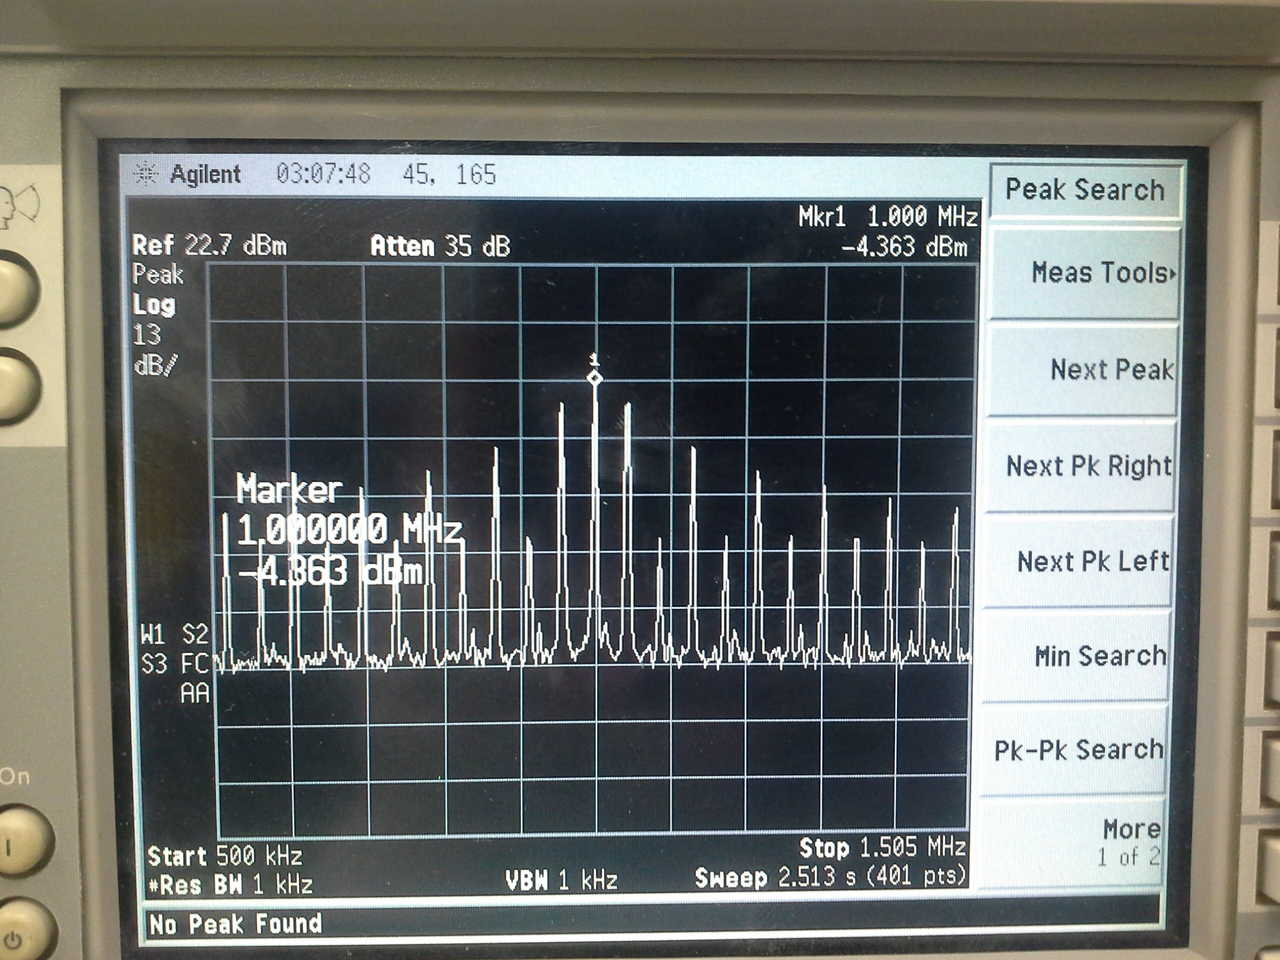
\includegraphics[scale=0.17]{../Grafiken/Frequenzspektrum_d_FreqModuliert_0.jpg}
		\caption{Grundfrequenz\label{fig:frequenzspektrum_d_freqmoduliert_0}}
	\end{subfigure}%
	
	\begin{subfigure}[t]{0.5\textwidth}
		\centering
		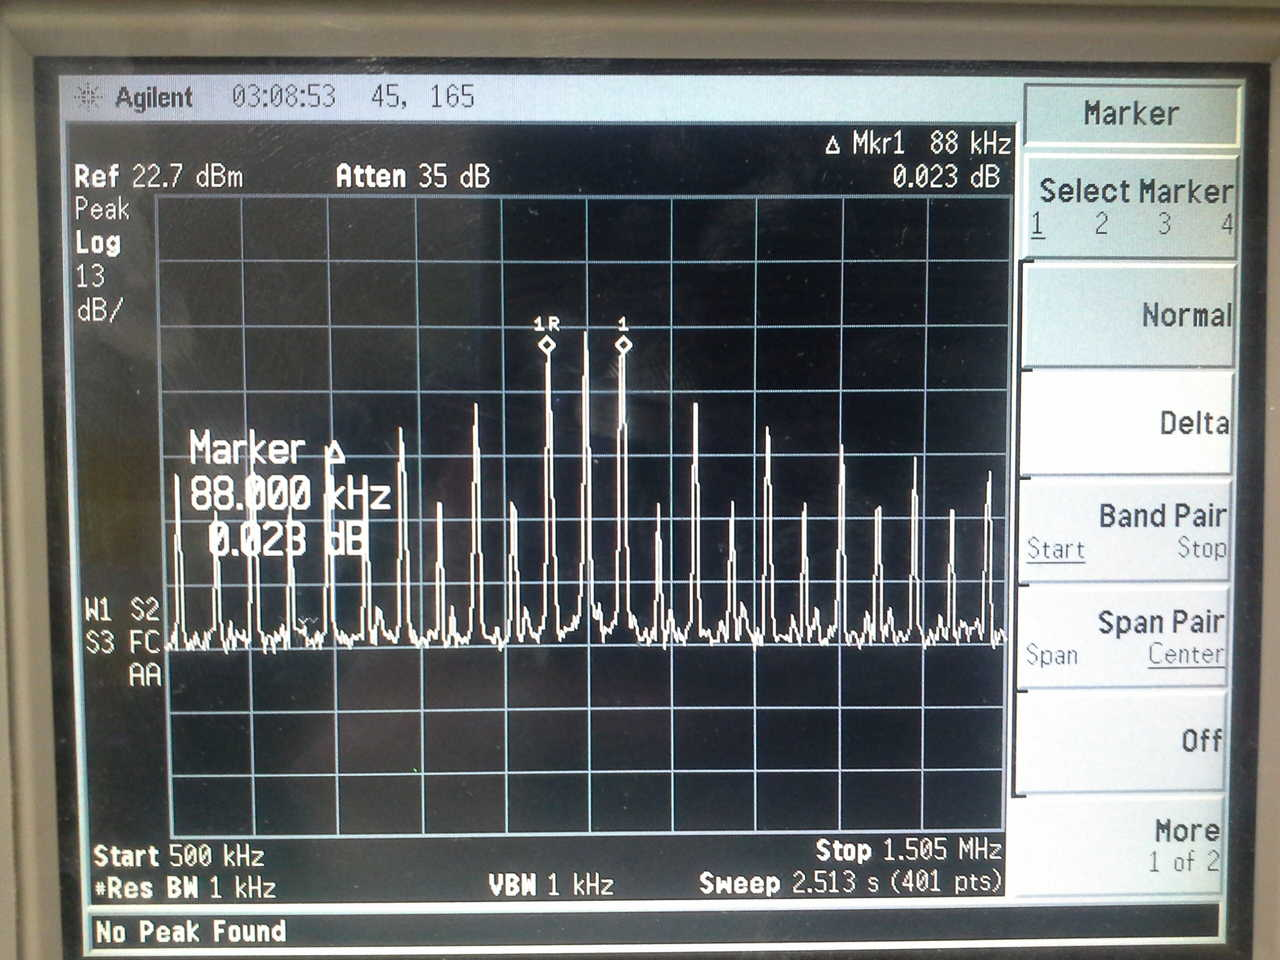
\includegraphics[scale=0.17]{../Grafiken/Frequenzspektrum_d_FreqModuliert_1.jpg}
		\caption{Frequenzdifferenz der ersten Seitenbänder\label{fig:frequenzspektrum_d_freqmoduliert_1}}
	\end{subfigure}%
	~
	\begin{subfigure}[t]{0.5\textwidth}
		\centering
		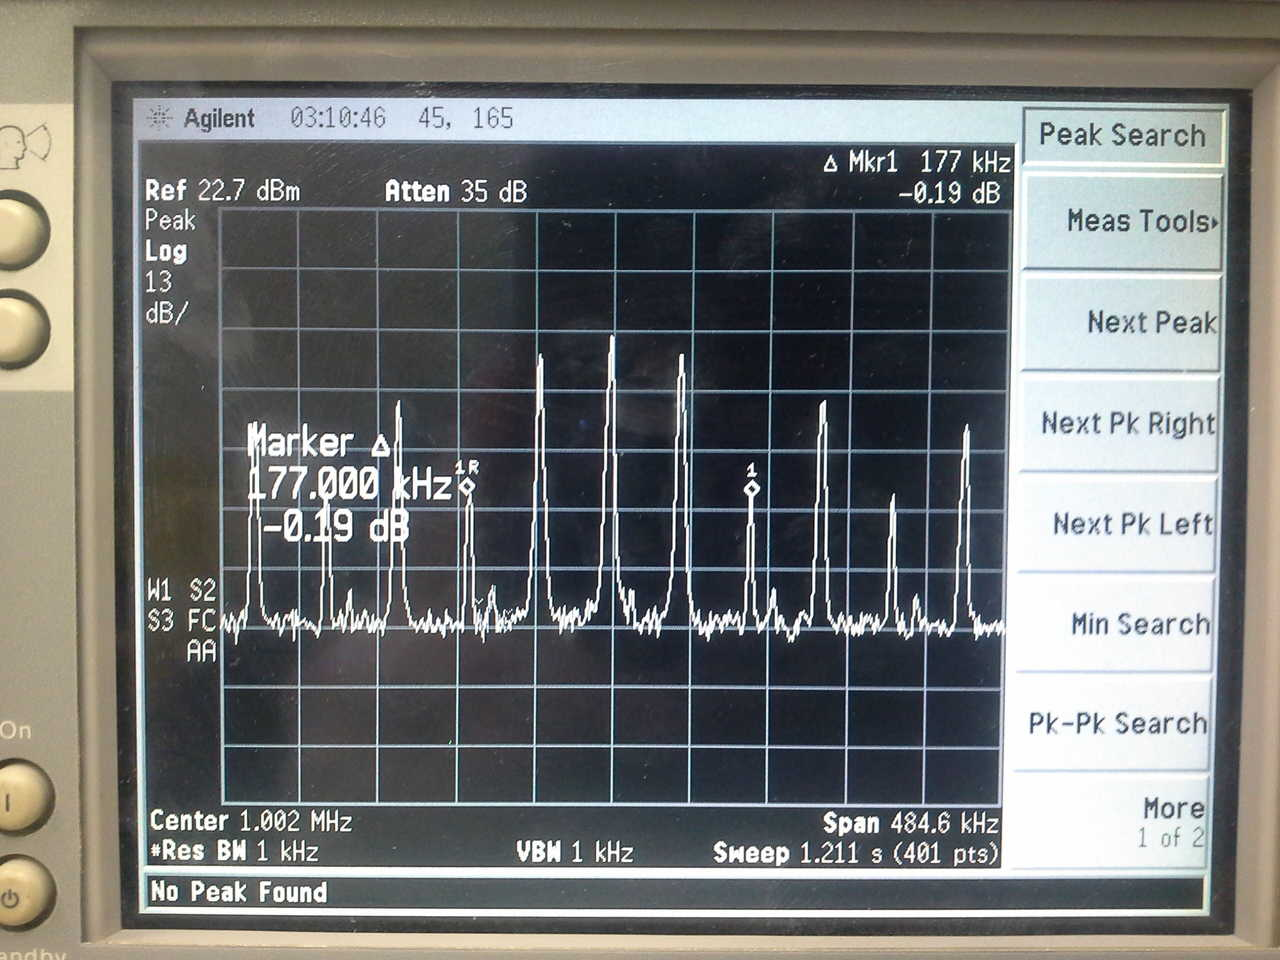
\includegraphics[scale=0.17]{../Grafiken/Frequenzspektrum_d_FreqModuliert_2.jpg}
		\caption{Frequenzdifferenz der zweiten Seitenbänder\label{fig:frequenzspektrum_d_freqmoduliert_2}}
	\end{subfigure}
	\caption{\label{fig:frequenzspektrum_d_freqmoduliert}}
\end{figure}
\FloatBarrier